% !TeX spellcheck = it_IT
%!TEX encoding = UTF-8 Unicode
%Author: Fulvio Frapolli
%Last revision: 06.09.2019
\documentclass[
%todo,
%answers,
finale,
%sectnum,
ssectnum,
%twocolumn,
]{DossierExMathIta}

\titolo[indice]{Database}
%\titolo{PAP1}
\author{CPT}
\date{2020}


%\pgfplotsset{AxisDefaults/.append style={width=\linewidth,}}
\tikzstyle{every node}=[font=\footnotesize] 
\renewcommand\partlabel{\arabic{partno})} %% Keep consistency in part numbering  with the screenshots

\makeatletter
\def\input@path{{esercizi/}}
%or: \def\input@path{{/path/to/folder/}{/path/to/other/folder/}}
\makeatother


\begin{document}
\setlength{\columnsep}{0.6cm}
\indice


\section{Insiemi}
\subsection{Numeri}
\begin{questions}

	\question

	\exonly{	Indica a quali insiemi appartengono i seguenti valori: }
	
	\begin{minipage}{\linewidth}
	\begin{multicols}{2}
		\begin{tabular}{|c|c|c|c|c|}
			\hline
			                & $ \mathbb{N}$ & $ \mathbb{Z}  $ & $ \mathbb{Q}$ & $ \mathbb{R} $ \\
			\hline
			     $ 4 $      &      \solonly{\checkmark }         &  \solonly{\checkmark }                &    \solonly{\checkmark }            &    \solonly{\checkmark }             \\
			\hline
			   $ -0.34 $    &               &                 &    \solonly{\checkmark }            &      \solonly{\checkmark }           \\
			\hline
			    $ -71 $     &               &      \solonly{\checkmark }            &    \solonly{\checkmark }            &   \solonly{\checkmark }              \\
			\hline
			$ \frac{3}{4} $ &               &                 &     \solonly{\checkmark }           &        \solonly{\checkmark }         \\
			\hline
			    $ \pi $     &               &                 &               &    \solonly{\checkmark }             \\
			\hline
			 $ \sqrt{2} $   &               &                 &               &    \solonly{\checkmark }             \\
			\hline
		\end{tabular}
		
		\begin{tabular}{|c|c|c|c|c|}
			\hline
			                       & $ \mathbb{N}$ & $ \mathbb{Z}  $ & $ \mathbb{Q}$ & $ \mathbb{R} $ \\
			\hline
			      $ 3.1415 $       &               &                 &    \solonly{\checkmark }            &      \solonly{\checkmark }           \\
			\hline
			    $ \sqrt{121} $     &  \solonly{\checkmark }              &    \solonly{\checkmark }              &   \solonly{\checkmark }             &   \solonly{\checkmark }              \\
			\hline
			  $ \frac{\pi}{2} $    &               &                 &               &   \solonly{\checkmark }              \\
			\hline
			    $ \sqrt{-4} $      &               &                 &               &                \\
			\hline
			$ \sqrt{\frac{3}{4}} $ &               &                 &               &    \solonly{\checkmark }             \\
			\hline
			 $ 2.\overline{342} $  &               &                 &    \solonly{\checkmark }            &    \solonly{\checkmark }             \\
			\hline
		\end{tabular}
		
\end{multicols}
\end{minipage}



\end{questions}


\subsection{Operazioni}
\begin{questions}


\question

\exonly{
Sono dati i seguenti insiemi:

\begin{multicols}{2}
	\begin{itemize}
		\item $A=\{1;2;3;4\}$ 
		\item $B=\{3,5,7,8\}$
		\item $P=\{0;2;4;6;8;10;...\}$ 
		\item $D=\{1;3;5;7;9;11;...\}$
	\end{itemize}
\end{multicols}


trovare: 
}

\begin{minipage}{\linewidth}
\begin{multicols}{2}
	\begin{parts}
		\part \exonly{$A\cap B$ } \solonly{$\left\lbrace 3  \right\rbrace $ }
		\part \exonly{$A\cup B$ } \solonly{$\left\lbrace 1;2;3;4;5;7;8  \right\rbrace $  }
		\part \exonly{$A\cup\mathbb{N}$ } \solonly{$\N $  }
		\part \exonly{$B\cap\mathbb{N}$ } \solonly{$B$ }
		\part \exonly{$A\cap D$ } \solonly{$\left\lbrace 1;3  \right\rbrace $  }
		\part \exonly{$(A\cup B)\cap P$ } \solonly{$\left\lbrace 2;4;8  \right\rbrace $  }
		\part \exonly{$(A\cap B)\cap P$ } \solonly{$\emptyset$ }
		\part \exonly{$B\cap P$ } \solonly{$\left\lbrace  8 \right\rbrace $  }
		\part \exonly{$A\setminus B$ } \solonly{$\left\lbrace  1;2;4 \right\rbrace $  }
		\part \exonly{ $\mathbb{N}^{*}\setminus A$ } \solonly{$\left\lbrace  5;6;7;\ldots \right\rbrace $  }
		\part \exonly{$\mathbb{N}\setminus P$ } \solonly{$D$ }
		\part \exonly{$P\cap D$ } \solonly{$\emptyset$ }
		\part \exonly{$A\cup(B\cap P)$ } \solonly{$\left\lbrace  1;2;3;4;8 \right\rbrace $  }
		\part \exonly{$A\cap(B\cap P)$ } \solonly{$\emptyset$ }
	\end{parts}
\end{multicols}
\end{minipage}

\question
\exonly{	Sono dati i seguenti insiemi:

\begin{multicols}{2}
	\begin{itemize}
		\item $A=\{-5;-2;3;6;8\}$
		\item $P=\{0;2;4;6;8;10;...\}$
		\item $B=\{0;2;4;10;14;22\}$
		\item $D=\{1;3;5;7;9;11;...\}$
		\item $C=\{3;4;5;6;7;8;9\}$
	\end{itemize}	
\end{multicols}

Indica se le seguenti espressioni sono vere o false: }

\begin{minipage}{\linewidth}
\begin{multicols}{2}
	\begin{tabular}{|l|c|c|}
		\hline
		& v & f  \\
		\hline
		$B\subset P$          & \solonly{\checkmark }    &    \\
		\hline
		$A\not\subset D$      & \solonly{\checkmark }    &    \\
		\hline
		$B\in\mathbb{N}$      &   &  \solonly{\checkmark }    \\
		\hline
		$2\in A$              &   &  \solonly{\checkmark }    \\
		\hline
		$\mathbb{N}\subset P$ &   &  \solonly{\checkmark }    \\
		\hline
		$(P\cap D)=\emptyset$      & \solonly{\checkmark }    &    \\
		\hline
	\end{tabular}
	
	\begin{tabular}{|l|c|c|}
		\hline
		& v & f \\ \hline
		
		$(B\setminus A)\subset P$           &  \solonly{\checkmark } &   \\ \hline
		
		$(C\cap P)\not\subset D$            &   & \solonly{\checkmark }  \\ \hline
		
		$(A\cup B)\subset\mathbb{N}$        &   &  \solonly{\checkmark } \\ \hline
		
		$(P\setminus B)\subset\mathbb{N}^*$ & \solonly{\checkmark }  &   \\ \hline
		
		$P\cup D\subset\mathbb{N}$          & \solonly{\checkmark }  &   \\ \hline
		
		$(A\cup P)\subset C$                &   &   \solonly{\checkmark }\\ \hline
	\end{tabular}
	
\end{multicols}
\end{minipage}



\end{questions}


\exnewpage



\section{Aritmetica}
\subsection{Priorità delle operazioni}
\begin{questions}
	
	
\question
\exonly{		
	Calcola senza aiutarti con la calcolatrice:
\begin{multicols}{3}
	\begin{parts}
		\part $ \dfrac{2}{3} + \dfrac{3}{4} = $
		\part $ \dfrac{7}{6} - \dfrac{5}{8} + \dfrac{4}{9} = $
		\part $ \dfrac{1}{15} - \dfrac{2}{5} + \dfrac{3}{25} = $
		\part $ \dfrac{2}{6} + \dfrac{5}{15} - \dfrac{12}{18} = $
		\part $ \dfrac{a}{3} + \dfrac{2}{5} - \dfrac{4}{3} = $
		\part $ \dfrac{1}{x} + \dfrac{3}{5} - \dfrac{3}{2x} = $
		\part $ \dfrac{\dfrac{1}{3} + \dfrac{1}{5}}{\dfrac{4}{15}-\dfrac{2}{6}} = $
		\part $ \dfrac{\dfrac{2}{3} \cdot (\dfrac{1}{6} + \dfrac{1}{2})}{\dfrac{3}{4}-\dfrac{3}{10}} = $
		\part $ \dfrac{2}{3} \cdot \dfrac{1}{5} + \dfrac{\dfrac{3}{2}}{\dfrac{7}{5}} = $
		\part $ \dfrac{4}{9} \cdot \dfrac{6}{10} + \dfrac{\dfrac{8}{30}}{\dfrac{6}{5}} = $
	\end{parts}	
\end{multicols} }
\solonly{Calcolatrice CAS}

\question
\exonly{
		Calcola senza aiutarti con la calcolatrice:
\begin{multicols}{2}
	\begin{parts}
		\part $ 2^3 \cdot 2^{-2} \cdot 2^4 \cdot 2^{-1} =$
		\part $ \dfrac{3^2\cdot 3^3}{3^4} = $
		\part $ \dfrac{5^3\cdot 5^{-2}}{5^4 \cdot 5^{-3}} = $
		\part $ \left(2^2\right)^2 \cdot \left(2^{-1}\right)^3 \cdot \left(2^2\right)^{-2} $
		\part $ \left(3^2\right)^{-1} \cdot \left(2^{-2}\right)^{-1} \cdot \left(6^2\right)^2 =$
		\part $ \left[\left(\dfrac{1}{5}\right)^{2}\cdot\left(\dfrac{1}{5}\right)^{3}\right]^{2}\cdot\left(\dfrac{1}{5}\right)^{-7} = $
		\part $ \dfrac{3^5 \cdot 2^4}{6^3} = $
		\part $ \dfrac{\left[\left(\dfrac{3}{4}\right)^{-1}\right]^{2} \cdot \left(\dfrac{2}{9}\right)^{-2}}{\left(\dfrac{1}{6}\right)^{-3}} = $
		\part $ \left\lbrace \dfrac{\left[\left(3^{2}\right)^{-1}\right]^{2}}{\left(\dfrac{1}{3}\right)^{-3}}\right\rbrace ^{-1} \cdot \left[\left(\dfrac{2}{5}\right)^{2} \cdot \left(\frac{5}{6}\right)^{2}\right]   = $
	\end{parts}
\end{multicols}
 }
	

\question
\exonly{Semplifica e calcola senza utilizzare la calcolatrice: }

%\exonly{
%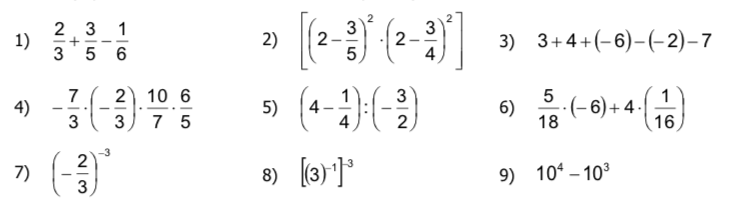
\includegraphics[scale=0.6]{test-form-1}
%
%}
\begin{minipage}{\linewidth}
	\begin{multicols}{2}
\begin{parts}
	\part
	\exonly{$\dfrac{3}{3}+\dfrac{3}{5}-\dfrac{1}{6}$ }
	\solonly{$\dfrac{11}{10}$ }
	
	\part
	\exonly{ $\left[ \left( 2-\dfrac{3}{5}\right) ^2 \cdot \left( 2-\dfrac{3}{4}\right) ^2 \right] $  }
	\solonly{$\dfrac{49}{16}$ }
	
	\part
	\exonly{$3+4+(-6)-(-2)-7$ }
	\solonly{$-4$ }
	
	\part
	\exonly{$-\dfrac{7}{3} \cdot \left( -\dfrac{2}{3}\right) \cdot \dfrac{10}{7} \cdot \dfrac{6}{5} $ }
	\solonly{$\dfrac{8}{3}$ }
	
	\part
	\exonly{$\left( 4-\dfrac{1}{4}\right) \div \left( -\dfrac{3}{2}\right) $ }
	\solonly{$-\dfrac{5}{2}$ }
	
	\part
	\exonly{$\dfrac{15}{18}\cdot\left( -6 \right) +4\cdot \left( \dfrac{1}{16}\right) $ }
	\solonly{$-\dfrac{17}{12}$ }
	
	\part
	\exonly{$\left( -\dfrac{2}{3}\right) ^{-3}$ }
	\solonly{$-\dfrac{27}{8}$ }
	
	\part
	\exonly{$\left[ \left( 3\right) ^{-1}\right] ^{-3}$ }
	\solonly{$27$ }
	
	\part
	\exonly{$10^4-10^3$ }
	\solonly{$9000$ }
\end{parts}
\end{multicols}
\end{minipage}

%\solonly{
%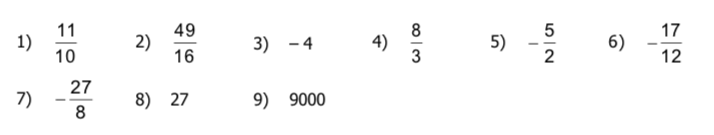
\includegraphics[scale=0.6]{test-form-1-sol}
%}

%\exnewpage

\begin{minipage}{\textwidth}	
\question
\exonly{
	Calcola senza aiutarti con la calcolatrice:
	

\begin{multicols}{2}
	\begin{parts}
		\part $ x - 2x + 3x - 4x + 5x - 6x =$
		\part $ a^2 + 2a -3a^2 +a = $
		\part $ a^2 \cdot a^3 = $
		\part $ \left(a^2\right)^2 + a\cdot a^3 - \left(a^6\right)^{-2} =$
		\part $ x^{-2} \cdot \left(x^2\right)^3 = $
		\part $ \dfrac{9 \cdot a^2 \cdot b^3 }{3 \cdot a^{-2} \cdot b^5} = $
		\part $ \dfrac{2 \cdot a^3 \cdot b^2 }{3 \cdot a \cdot b^4} \cdot \dfrac{a+b}{a}  = $
		\part $ a\left(a(a^{-1}+1) + a(a-1)\right) =$
\end{parts}

\end{multicols}

 }\end{minipage}


\end{questions}

\subsection{Notazione scientifica}
\begin{questions}
	
\question
\exonly{
		Esprimi la tua altezza in notazione scientifica
\begin{multicols}{2}
	\begin{parts}
		\part in metri
		\part in centimetri
		\part in millimetri
		\part in chilometri
		\part in pollici ($\SI{1}{in}=\SI{2.54}{cm}$)
		\part in piedi ($\SI{1}{ft}=\SI{12}{in}$)
	\end{parts}
\end{multicols}
 }

\question
\exonly{
		Calcola senza aiutarti con la calcolatrice:
\begin{parts}
	\part $\num{2e3} + \num{5e2} +\num{3e1}=$
	\part $\num{3e3} + \num{5e-2} +\num{2e-1} + \num{6e1} + \num{4e0} + \num{9e2} + 7 \times 10^0=$
	\part $ \num{12e3} \times \num{2e-3} \times \num{3e-6} =$
	\part $ \dfrac{\num{12e3}+ 500}{\num{5e6}} = $
	\part $ \dfrac{\num{2e-2} \times\num{3e1} \times\num{4e2}}{\num{4e2} \times\num{6e-3} \times\num{2e1}} =$
	
\end{parts}
 }
\question
\exonly{ Calcolare le seguenti espressioni ed esprimere il risultato in notazione scientifica }

\begin{minipage}{\linewidth}
	\begin{multicols}{2}
\begin{parts}
	\part
	\exonly{ $\num{0.5e-1 }$ }
	\solonly{$ \num{5e-2}$ }

	\part
	\exonly{ $\num{-6.5e-5} -\num{3.5e-7} $ }
	\solonly{$-\num{6.535e-5} $ }
	
	\part
	\exonly{$\left(3 \cdot 10^{-2}\right)\left(4 \cdot 10^{-1}\right)$ }
	\solonly{ $\num{1.2e-2}$ }
	
	\part
	\exonly{$8^{2} \cdot 10^{-2}$ }
	\solonly{$\num{6.4e-1} $ }
	
	\part
	\exonly{ $200 \cdot 10^{4}$ }
	\solonly{$\num{2e6}$ }
	
	\part
	\exonly{$\left(5 \cdot 10^{-4}\right)\left(0,7 \cdot 10^{-8}\right)$ }
	\solonly{$\num{3.5e-12} $ }
	
	\part
	\exonly{$\left(7 \cdot 10^{-7}\right)^{2}$ }
	\solonly{$\num{4.9e-13}$ }
	
	\part
	\exonly{ $\left(3^{2} \cdot 10^{-6}\right)^{2} \cdot 10$ }
	\solonly{$ \num{8.1e-10} $ }
	
	\part
	\exonly{$10^{4}-10^{3}$ }
	\solonly{$\num{9e3}$ }
	
	\part
	\exonly{ $\left(0,4 \cdot 10^{-4}\right)(0,8) \cdot 10^{-4}$}
	\solonly{$\num{3.2e-9}$ }
	
	\part
	\exonly{$10^{5}-10^{-5}$ }
	\solonly{$\num{9.999999999e4}$ }
	
	\part
	\exonly{$\frac{\left(4^{2}\right)^{-2} \cdot 10^{-3}}{4^{-2} \cdot 10^{-8}}$ }
	\solonly{ $\num{6.25e3}$ }
	
	\part
	\exonly{$-\num{4.2e-3}+\num{4.2e5}$ }
	\solonly{$\num{4.199999958e5} $ }
\end{parts}
\end{multicols}
\end{minipage}

\question
\exonly{
		Calcola:
\begin{multicols}{2}
	\begin{parts}
		\part $ \SI{5.3}{cm} - \SI{3.2}{mm} = $ 
		\part $ \SI{43.5}{cm} \cdot \SI{9.3}{mm} = $ 
		\part $ \SI{9.2}{cm^2} + \SI{123}{mm^2} = $ 
		\part $ \dfrac{\SI{430}{mm^2}}{\SI{3.2}{cm}} = $
		\part $ \SI{3.2}{k\ohm} \cdot \SI{15}{mA} = $
		\part $ \dfrac{\SI{12}{V}}{\SI{60}{mA}} = $
	\end{parts}
\end{multicols}
 }

\question
\exonly{
		Esprimi le seguenti frazioni in notazione scientifica e tecnica
\begin{multicols}{2}
	\begin{parts}
		\setlength\itemsep{1em}
		\part $\dfrac{5}{8}$=
		\part $\dfrac{724}{5}$=
		\part $\dfrac{11562}{470000}$=
		\part $\dfrac{123456}{7}$=
		\part $\dfrac{12}{16500}$=
		\part $\dfrac{146}{2420}$=
	\end{parts}
\end{multicols}
 }


\end{questions}





\end{document}